%
%   Managing input data
%
\subsection{Managing input data} \label{subsec:RNN}
As discussed in the introduction, the purpose of the work is to analyse several different RNN models, measure the performance, and determine the most promising direction for further enhancing Neural Network models' integration into an embedded device.
Although the perfect replication was impossible due to a lack of details and actual battery data used by different authors, all models were implemented based on the provided information.
All missing aspects were assumed based on ML's standard methods at the time of their writing.
Deriving from Table~\ref{tab:review}, Table~\ref{tab:experiment} compiles models, which will be evaluated in this work.
It provides details of 7 different implementations, which vary in structure and learning process but share the same training, validation, testing and performance measurement procedures.

%
%
The structure and cell type define the number of layers of particular cell types with the total number of neurons evenly shared across layers.
The statefulness parameter describes the model ability to preserve its' current state for the next set of input parameters.
Based on that, the input amount of samples become flexible by the requirement of adding only a single sample at a time upon their arrival, instead of waiting until the fixed amount has accumulated into a fixed-size time window.
The optimiser selection was based on the derivative calculation algorithms only.
Other alternatives, like differential evolution, are beyond the scope of research.
Finally, "Extension" defines the model's specific detail, which distinguishes it against the others.

%
%
Thus the specifics of each algorithmic aspect will be defined further~\ref{subsec:dataset},~\ref{subsec:structure}:
\begin{enumerate}
    \item Data shape for each state type
    \item Model structure and difference between GRU and LSTM
    \item Each optimisation algorithm and hyper-parameters selection
\end{enumerate}
\begin{table*}[h]
    \renewcommand{\arraystretch}{1.3}
    \caption{Testing models summary.}
    \centering
    \label{tab:experiment}
    \resizebox{\textwidth}{!}{
    \begin{tabular}{l|l|c|c|c|c|c|l}
        \hline\hline \\[-4mm]
        \multirow{2}{ 4em }{\#} &
        \multirow{2}{ 4em }{Structure \& Cells} &
        \multirow{2}{ 4em }{State$-$ } &
        \multicolumn{4}{ c|}{Optimiser Learning Rate} &
        \multirow{2}{ 4em }{Extension} \\
        \cline{4-7}
        &                       &         & Adam  & Nadam & SGDw/M\footnote{Stochastic Gradient Descent with Momentum} & AdaMax &           \\
        \hline
        1 & 1 $\times$ LSTM (500) & $-$less & 0.001 &       &        &        &           \\
        2 & 1 $\times$ GRU (560)  & $-$less &       & 0.001 &        & 0.0005 & Ensemble  \\
        3 & 1 $\times$ LSTM (520) & $-$less & 0.001 &       &        &        & Attention \\
        4 & 2 $\times$ GRU (60)   & $-$ful  &       &       & 0.001  &        & Momentum (0.3)\\
        5 & 1 $\times$ GRU (500)  & $-$less & 0.0001 &       &        &        & RoAdam\\
        6 & 2 $\times$ LSTM (250)   & $-$less  & 0.001 &       &        &        &           \\
        \hline\hline
    \end{tabular}
    }
\end{table*}


%
%
\subsection{Dataset description and generator} \label{subsec:dataset}
Recurrent Neural Network is a subclass of NN, proven effective in weather or stock prices forecasting.
This method learns by recognising a pattern within sequential data input, thus predicting the future outcome.
It makes the following approach applicable to almost any type of time series dependant problem~\cite{anton_battery_2013}.
Classical RNN consists primarily of three layers, represented in Figure~\ref{fig:RNN-structure}.
The two vectors or matrices define the Input and Output Layers.
The general description of a single input X and an output Y samples are represented by Equations~\ref{eq:xy-matrix}.
$V, I, T, SoC$ represent Voltage (V), Current (A), Temperature (\textdegree{}C) as input features, and percentage of State of Charge (between 0 and 1) as output.
All samples are equally time distributed, and the t represents the number of input time steps at a time.
\begin{equation}
    \textbf{X} \left (n  \right ) = 
    \begin{Bmatrix}
        V \left (0  \right ) & V \left (1  \right ) & ... & V \left (t  \right )\\ 
        I \left (0  \right ) & I \left (1  \right ) & ... & I \left (t  \right )\\ 
        T \left (0  \right ) & T \left (1  \right ) & ... & T \left (t  \right )\\
    \end{Bmatrix}
    \\ \textbf{Y} \left (n  \right ) = 
    \begin{Bmatrix}
        SoC \left (t  \right ) 
    \end{Bmatrix}
\label{eq:xy-matrix}
\end{equation}

%
%
For dataset generation of training and testing purposes, data is combined in a 3-dimensional matrix using windowing techniques as per Figure~\ref{fig:Windowing3f}, where $s$ represents the step between each window, less than the number of input time steps.
The optimum size of the windows for stateless models, obtained by Chemali et al.~\cite{Chemali2017}, will be 500 samples.
Figure~\ref{fig:chemali-accuracy} plots his findings in an accuracy plot over a size of time windows.
The shape demonstrates the root square polynomial, which indicates infinite growth towards zero.
Any more significant matrices will lead to an increase in computation time but an insignificant difference in performance.
All stateful models used the same windowing technique to keep data generation simple but with a sample size of 1.
The state reset for stateful models happens at the end of every dataset, allowing a batching mechanism to speed up the training process.
For example, 12 datasets of discharge process with similar Voltage, Current and the State of Charge, but different temperatures at a time $t$ can be treated as a single batch.
The statefulness of a model preserves the state at index $i$ to the same index in the next batch~\cite{zhu_statefulnes_tfdocs_2020}.
\begin{figure}[htbp]
    \centering
    \includesvg[width=\linewidth]{II_Body/images/chemali_accuracy.svg}
    \caption{SoC estimation accuracy of LSTM-RNN with various network depths in time by Chemali et al.~\cite{Chemali2017} in plot representation.}
    \label{fig:chemali-accuracy}
\end{figure}
%%%
% For the process of training for Stateful models speeding up, all data can be separated by batches \textit{b}, for each batch representing a different temperature category, creating a 4-dimensional matrix.
% \textit{f} defines the number of features as per Voltage, Current and Temperature.
% \textit{b} and \textit{s} were kept as the size of 1 for all scenarios to minimise resource consumption and simplify performance validation.
% Equation~\ref{eq:XY-shape} represent the final shape for Input data.
% The output shape for both Stateful and Stateless models remains the same.
% \begin{equation}
%     \begin{split}
%         X_{shape} = (n, b, t, f) & => (n, t, f) - Stateless \\
%                                  & => (n, 1, f) - Stateful \\
%         Y_{shape} = (n, b, 1) \ \ &=> (n, 1)
%     \end{split}
%     \label{eq:XY-shape}
% \end{equation}
%One of the first methods of SoC Estimation by Chemali \textit{et al.}~\cite{Chemali2017} proved that 500 input time-steps produced the most efficient results, any further grow made insignificant impact.
%The same value used in this article. \\

%
%
The value of SoC has been calculated from the difference between charge and discharge capacity.
Values were rounded to 2 decimal places and kept in the range of 0 and 1 using min-max normalisation to reduce error in estimation.
Since there is no way to directly obtain the battery's accurate charge practically during a run, output SoC is excluded from the time-series model's input feature, unlike any classic examples of usage Time-Series estimations.
The trainable model has to distribute weights across inputs and still develop a charge's close estimate.
All input samples were taken through normalisation by the mean and standard deviation across all input files with the same values, simplifying model weights acquiring and speeding up the training process.
It is important to note that the normalisation values of mean and standard deviation from a training dataset are applied to both validation and testings sets.

%
%
The training process was conducted through all datasets for a single battery testing profile and validated on a single cycle (less or around 20\% of the entire set).
Final tests for a model performance were conducted against an entire set of two remaining profiles separately.
\begin{figure}[htbp]
    \centering
    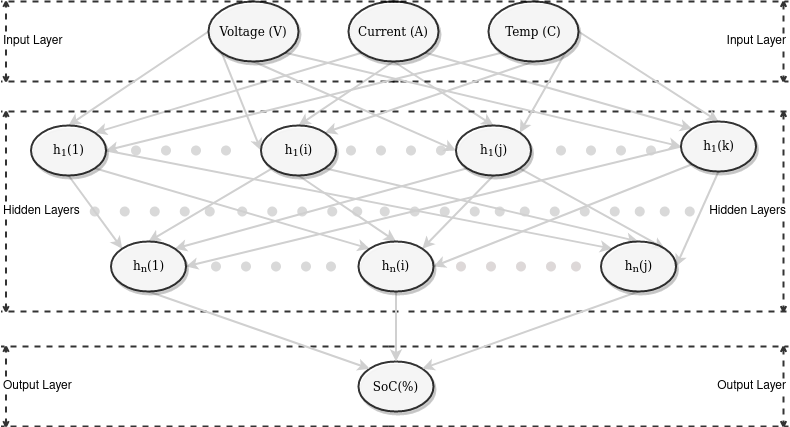
\includegraphics[width=\linewidth]{II_Body/images/SoC-RNN.png}
    \caption{Universal structure of RNN for SoC estimation.}
    \label{fig:RNN-structure}
\end{figure}
\begin{landscape}
    \begin{figure}[ht]
        \centering
        % 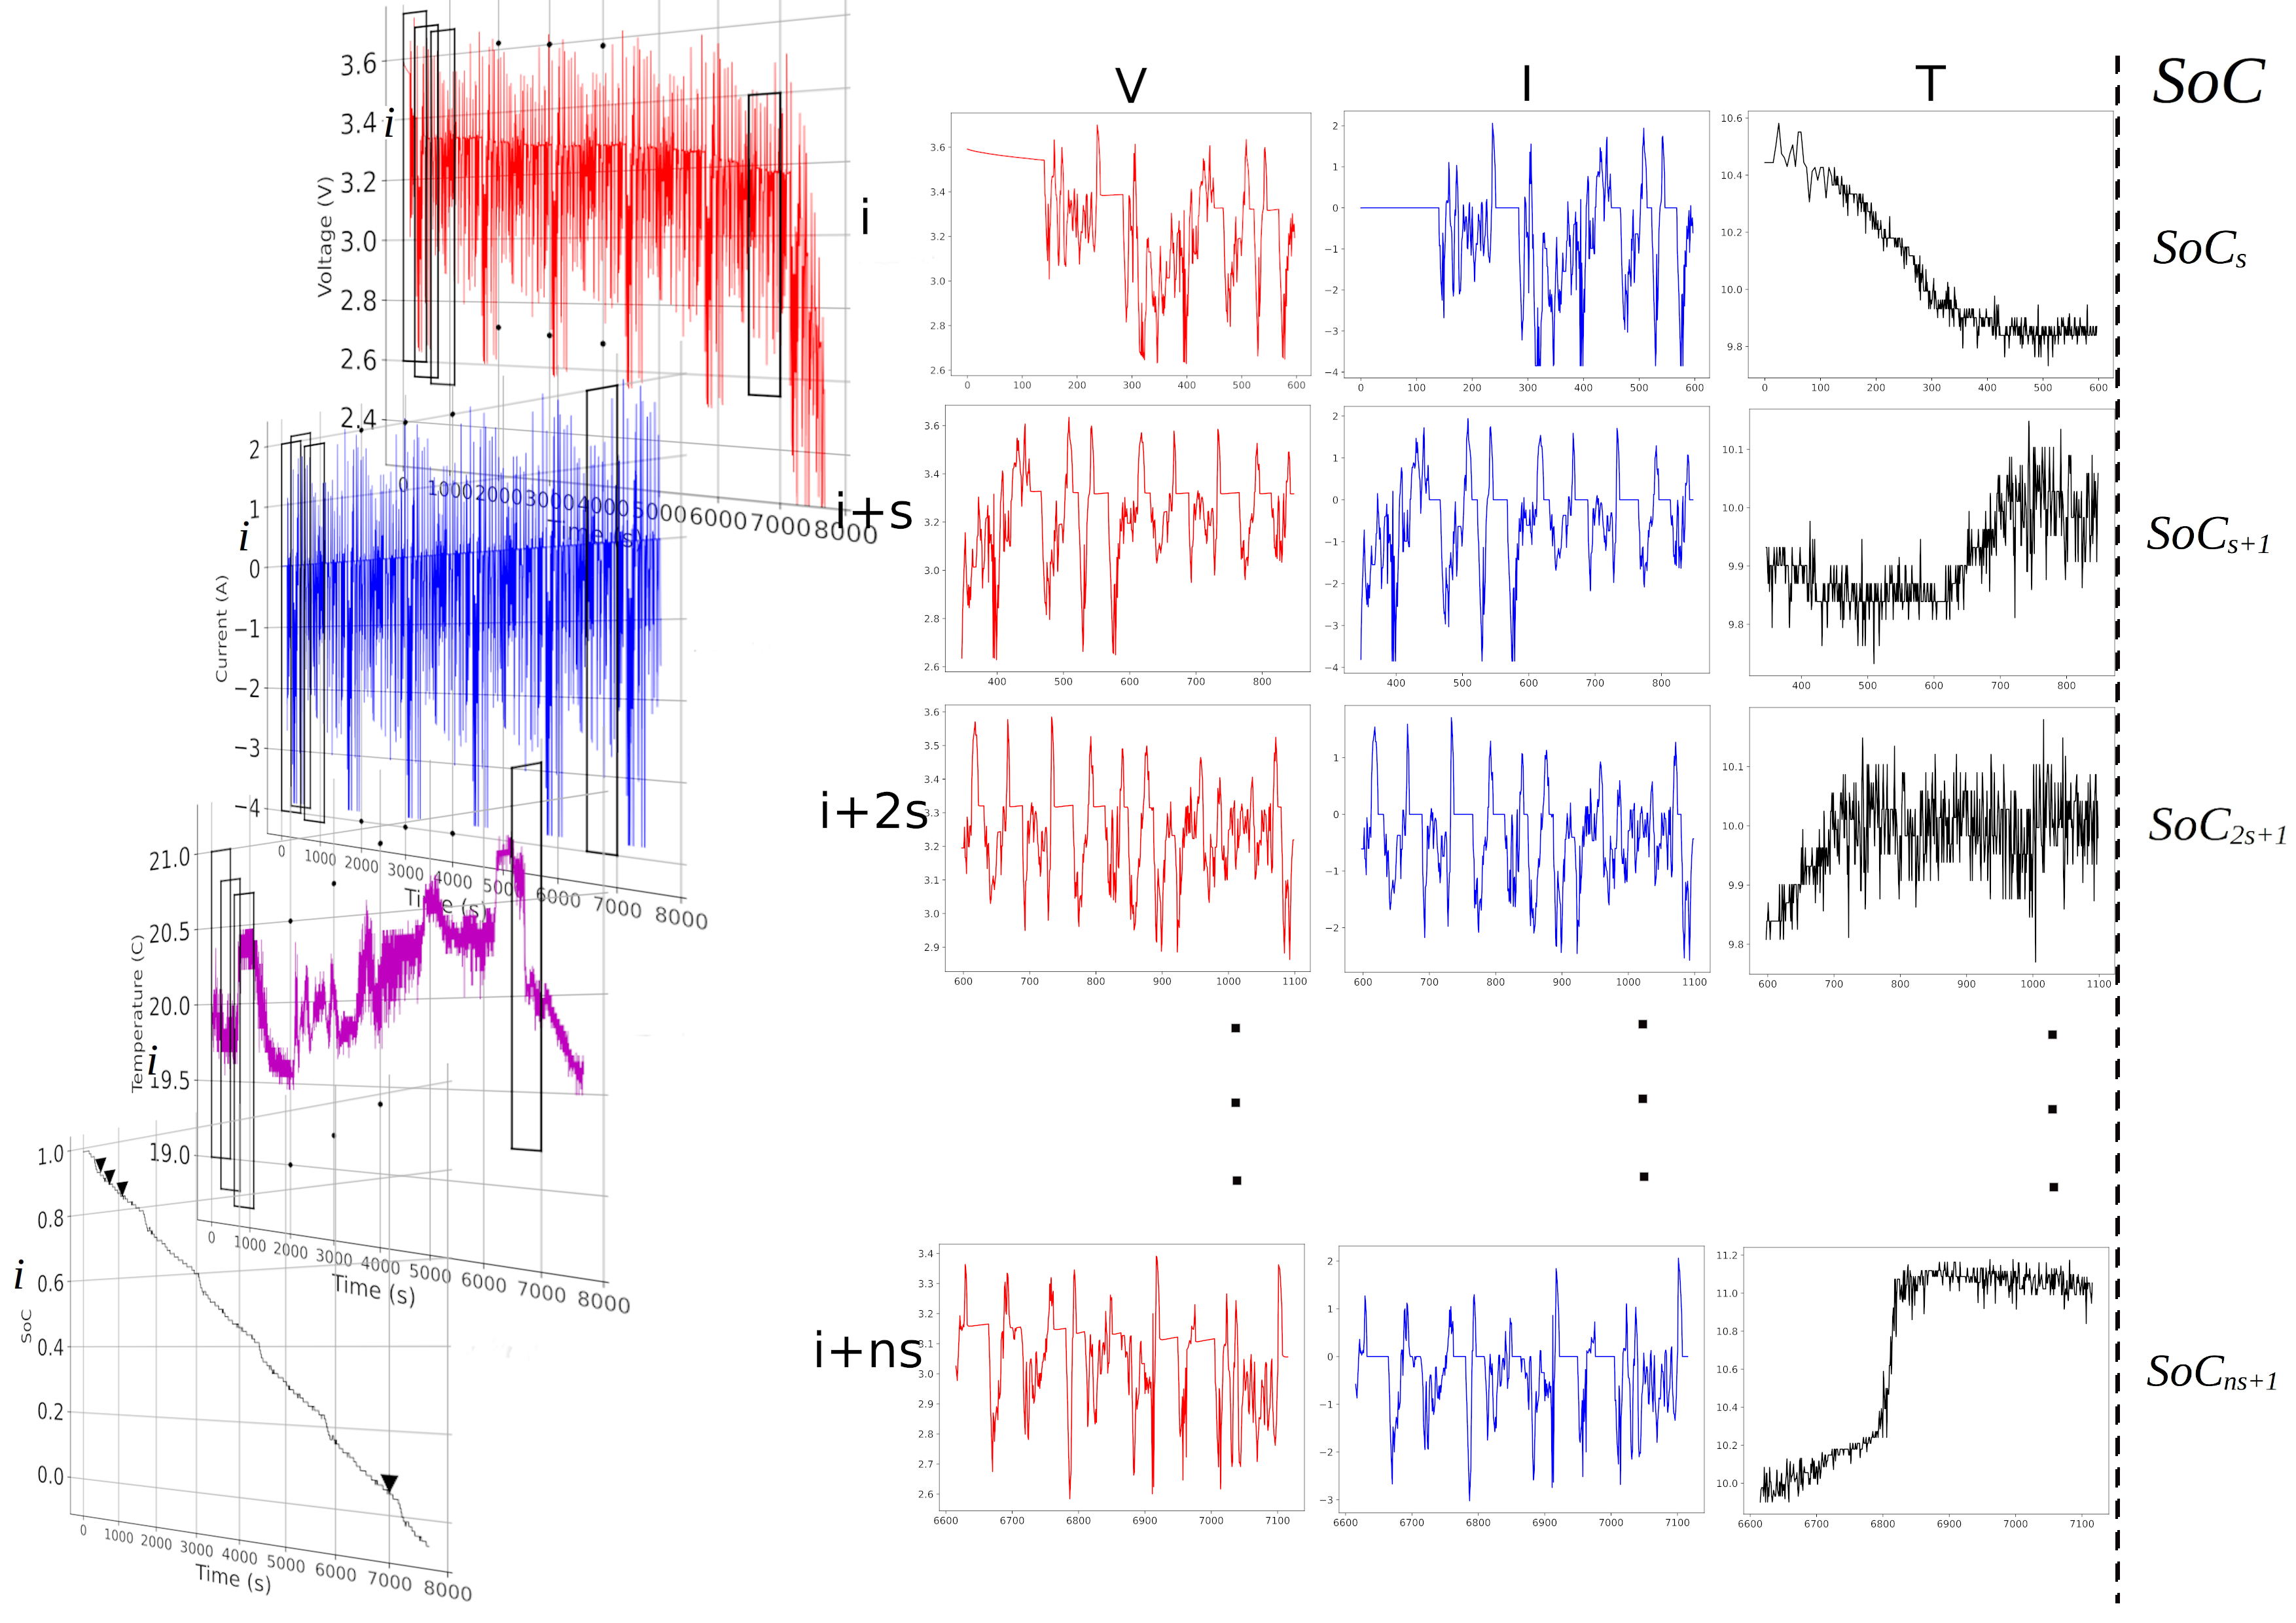
\includegraphics[width=0.9\linewidth]{II_Body/images/Windowing3D-3.jpg}
        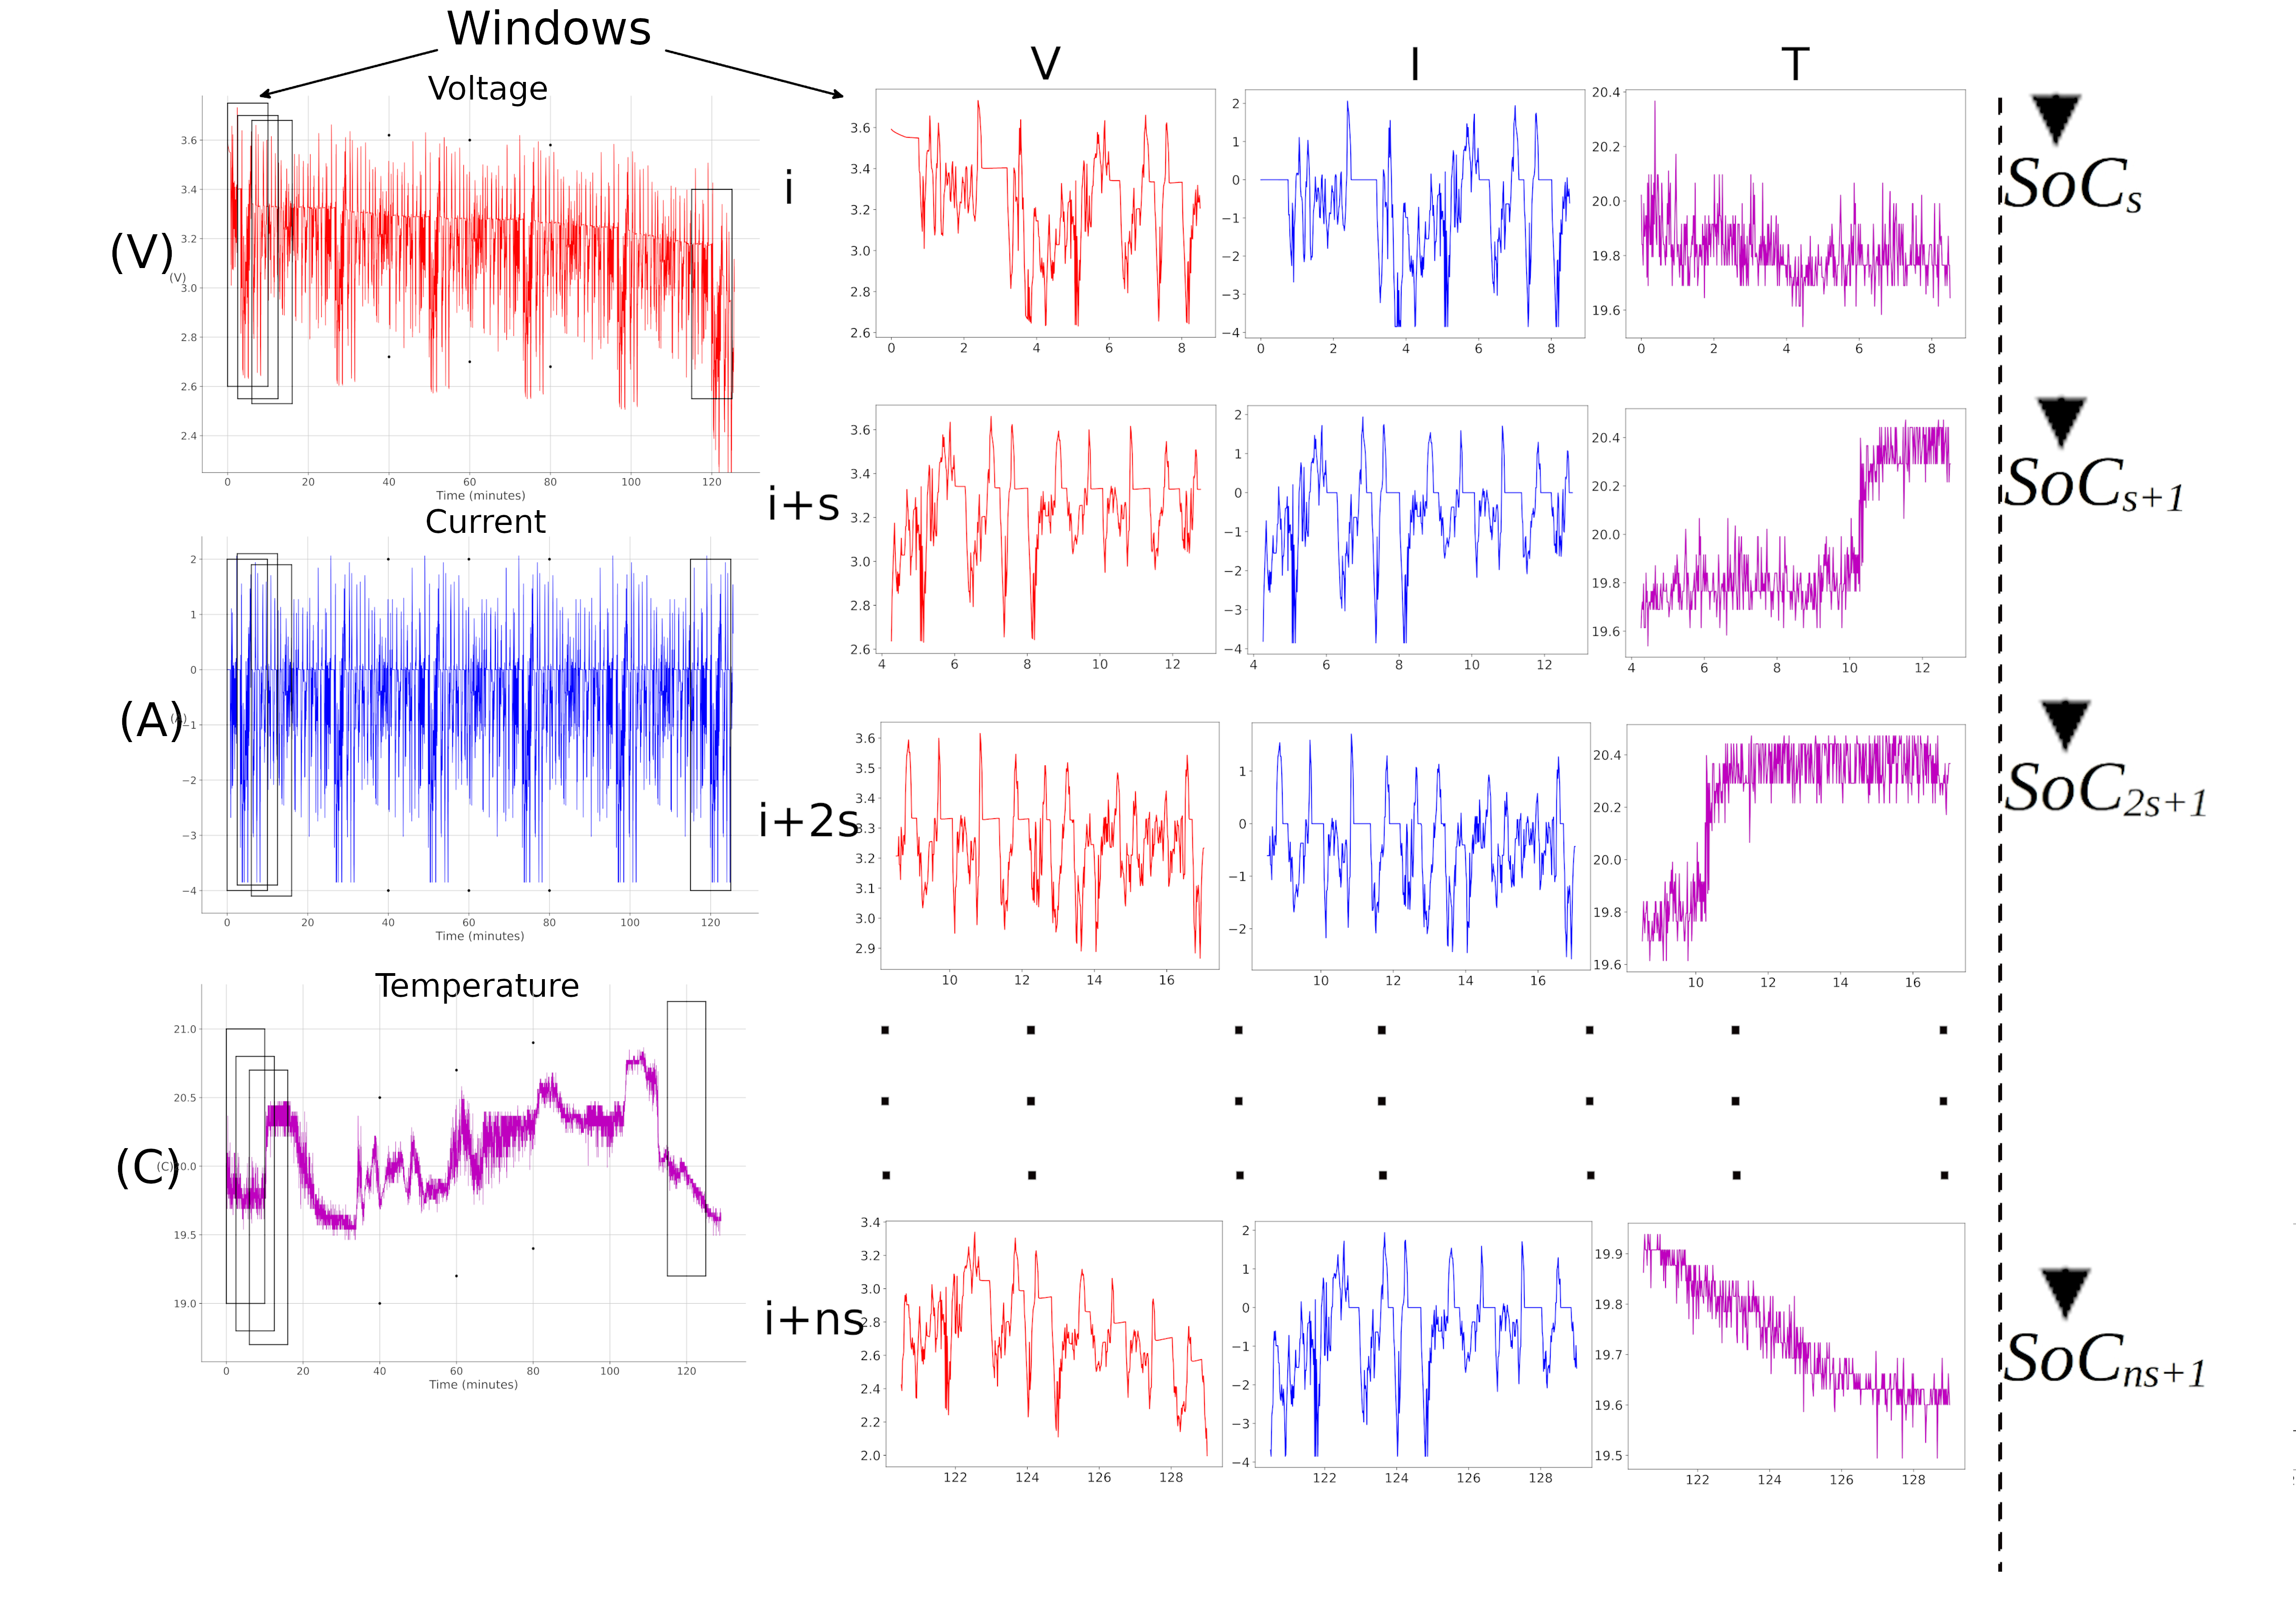
\includegraphics[width=\linewidth]{II_Body/images/windowing3f-A3.jpg}
        \caption{Data Windowing scheme. For visualisation purposes, the $s$-step has been used as 250 seconds, which is different from actual implementation. Initial index $i$ was kept as a value close to the beginning of the data, around zero.}
        \label{fig:Windowing3f}
    \end{figure}
\end{landscape}
%
%   Model Structure
%
\subsection{Model structure} \label{subsec:structure}
The general summary model structure is represented in Figure~\ref{fig:RNN-structure}, with three feature inputs and a single output.
The number of hidden layers will be dependant on the authors' implementation.
Since the output consists of only a single sample, it is defined by a fully connected layer - a dense layer with a single neuron.
In case if the article did not specify the number of neurons per layer, the following equations has been used to get the initial raw estimation~\cite{eckhardt_choosing_2018}:
\begin{equation}
    \begin{split}
        N_h &= \frac{N_s}{ a \left(N_i+N_o \right)} \ \ OR \ \ N_h = \frac{2}{3}\left(N_i+N_o \right) \\
        N_i &\rightarrow \text{Number of input neurons} \\
        N_o &\rightarrow \text{Number of output neurons} \\
        N_s &\rightarrow \text{Number of samples in training data set} \\
        \alpha &\rightarrow \text{An arbitrary scaling factor 2(5)-10}
    \end{split}
\end{equation}
%**Contrary with Hidden Layers as per their name, they obey only internally defined logic and connections.
%**That is why models are stable and reliable once created, cannot be changed, only retrainable with different data.
%A standard Hidden layer, consisting of fully connected neurons, called a Dense Layer.
%A standard Hidden layer, consisting of fully connected neurons and only one or none activation function, called a Dense Layer.
%Within each cell of a Dense layer lies a single activation function.

%An Output Layer gets created from Dense Layer and commonly with no Activation function.
%: \textit{Simple, Exponential or Rectified Linear; Sigmoid and Hyperbolic Tangent functions}. \\
% \begin{itemize}
%     \item \textit{linear} - Simple Linear function
%     \item \textit{elu} - Exponential Linear function
%     \item \textit{relu} - Rectified Linear unit function
%     \item \textit{sigmoind} - Sigmoid function $sigmoid(x) = 1/1(1+exp(-x)$
%     \item \textit{tanh} - Hyperbolic Tangent function $$
% \end{itemize}

%
%
There are several activation functions for those layers widely used in machine learning libraries for time series problems~\cite{amidi_cs_2018}.
For the SoC prediction problem, all authors used the same function.
It also was experimentally confirmed that the best one for all hidden layers is the hyperbolic tangent function, Equation~\ref{eq:tanh}.
The output layer does not use the same logic, and no activation gets applied.
A dropout layer technique with a 20\% cut-off has been applied to all hidden layers to prevent data overfitting over long training periods.
\begin{equation}
    tanh(x) = \frac{sinh(x)}{cosh(x)}=\frac{e^x-e^{-x}}{e^x+e^{-x}}
    \label{eq:tanh}
\end{equation}
%
%
%The common usage of Dense layer in this paper is the Output Layer with no activation functions and with single neuron representing single output SoC value.
%To apply multiple different without overcompicating neurons a multiple bunch of layers with different or the same number of neurons or activations functions gets applied.
%The more Hidden layers network contains - the deeper and computationally complex a network becomes, which also referred as Deep Neural Networks. 

% Choosing the number of neurons for a first Hidden Layer does not have a golden rule.
% For this article, following formula helps to make a good initial estimate based on Number samples, Inout and Output.\\
% \textbf{Equation}\\
% A common practice is to narrow each following Neurons by 2 from previous one, to make a more accurate capture.
% To avoid overfitting data, except for data normalization and Input sample shuffeling in stateles models, a Dropout technue gets applied.
% Tensorflow has an intermnal implementation of Dropoout for GRU and LSTM layers. A value of 0.2 (20\%) applied to all RNN layers to minimizze overfitting possibility.

%
% Requires editing below
The efficiency of an RNN over time series problem is defined by the ability of the neurons to store memory as an internal state.
With time, the memory of long passed samples may fade away.
The problem is called vanishing gradient when the value to update network weights shrinks as it propagates through time~\cite{rasifaghihi_predictive_2020}.
Long-term dependencies do not get captured since layers with a slight gradient do not significantly affect the system due to insufficient weight change~\cite{rasifaghihi_predictive_2020,hochreiter_vanishing_1998}.
The more complicated structures of neurons tend to solve that problem.
% The gradient is the value used to update Neural Networks’ weight.
%"Therefore, layers that get a small gradient do not learn and they cause the network to have short-term memory."
% https://www.bioinf.jku.at/publications/older/2304.pdf
%"With gradient based learning methods the current error signals has to 'flow back in time' over the feedback connections to past inputs for building up an adequate input storage. Long-term dependancies are hard to learn because of insufficient weight changes."

%
%
There are two commonly used Recurrent Neural Network, which utilises memory cells: Gated Recurrent Unit (GRU) and Long Short-Term Memory (LSTM) with possible extensions implemented by articles' authors.
The GRU implementation will be used as a stateful technique by preserving a state from batch to batch with a single sample at a time.
The LSTM will take a stateless approach, providing a fixed number of timestamps at a time.
%Implementation of the model based on simple RNN using multi layer Dense(X) networks.~\cite{lees2010theoretical}
%A very basic version of Recurrent Neural Network consist of very basic layers with some amount of neurons.

% \subsubsection{Implementation}
%     The input data for a network has been created using Windowing technique, where \textbf{216k} sample of battery data, consisting of State Of Charge only were separated on 500 sample windows.
%     As a results, model outputs a single sample as SoC at next Time Step. Using Tensorflow library and calculating number of Neurons using recomended formula \\
%     \textbf{THIS IS THE BEST PLACE FOR IT}. No other places suites as much.
%     The strcuture of the model ha\subsection{Training and Validation}

%s the following form. (Few Dense Layers+Dropount).
%     A Dropout layer has been used to prevent data overfitting. The selection of activation functions has been done through the properties of the data, which model has to fit in and multiple trials.
% \subsubsection{Observation}
%     A simple Recurrent Neural Network has proven itself effective with simple Linear problems. However, with battery state of charge it is unable to capture complicated features like transition between Discharge and Charge or process of Constant-Voltage Constant-Current charging. In the application of battery utilisation inside Electrical Vehichle, this approach can be used only with some additional logic, such as Kalman Filters.
%     The best approach is to introduce more information about battery state and use more complicated version of Time Series capable to memorise feature with time, such as LSTM~\ref{sec:LSTM} and GRU~\ref{sec:GRU}.
%     The results of the prediction discussed in Section~\ref{sec:results}.
%\subsection{Stateful Gradient Recurrent Unit (GRU) Algorithms and Implementations} \label{subsec:GRU}
%\subsection{LSTM with Attention}\label{sec:lstm-attention}
LSTM and GRU models made the most comonly used implemtation of Time -series predictions. TadeleMamo2020 research was intended to determine waknesses and improve the model introducing addition techniques into the default structure of training model***. \\
THe attention mechanissm used in ... \\
THe intention was to capture ... \\
\subsection{Implementation}
    Attention layer implementation was taken from \textbf{refernece} github repositry of ....
    
Implementation of the model based on TadeleMamo 2020 as the most recent and how to implement improvement to the model to make it better. Gracefully transition idea from here to my model, it is similar.
